\documentclass{article}
\title{Ant Colony Optimisation for the Travelling Salesman Problem}
\author{Dylan Galea}

\usepackage{cite}
\usepackage{amsmath}
\usepackage{amsthm}
\usepackage{amssymb}
\usepackage{physics}
\usepackage{tikz}
\usetikzlibrary{arrows.meta,automata,positioning}

\newtheorem{definition}{Definition}[subsection]
\newtheorem{theorem}[definition]{Theorem}
\newtheorem{lemma}[definition]{Lemma}
\newtheorem*{remark}{Remark}
\newtheorem{example}[definition]{Example}

\begin{document}
\maketitle
\newpage
\tableofcontents
\newpage
\section{Introduction}
Before defining the Travelling Salesman Problem and proving properties about it, a number of graph theoretic concepts must first be defined. Therefore, what follows is a sub-section that introduces a number of graph theoretic concepts which are required for the Travelling Salesman Problem.
\subsection{Some Graph Theory}
Graph theory is the study of the structure called a graph. A graph can be defined formally as shown in definition \ref{Graph} below.
\begin{definition}[Graph]
\label{Graph}
A graph G is a pair (V,E) were V is any non empty finite set called the set of vertices of G, and E $\subseteq$ \{$\{u,v\}$ $:$ u,v $\in$ V and u $\neq$ v\} is called the set of edges of G {\normalfont{\cite{black_tanenbaum_2017}}}. A graph G defined by the pair (V,E) is denoted by G(V,E) or G.
\end{definition}
A graph defined using definition \ref{Graph} is called an undirected graph. There is also the concept of a directed graph were $\mathit{E}$ $\subseteq$ \{(u,v) $:$ u,v $\in$ V and u $\neq$ v\} \cite{black_tanenbaum_2017}. However, in this thesis it can be assumed that any graph that will be considered is undirected unless otherwise stated. It can also be assumed that there are no edges between same vertices unless otherwise stated. The discussion will now proceed by introducing more graph theoretic terminology, along with examples for these terminologies.\\
\\When 2 vertices are joined by an edge, they are said to be adjacent. This is defined formally in definition \ref{adjacent} below.
\begin{definition}
\label{adjacent}
Given a graph G(V,E), $\forall$ u,v $\in$ V, u and v are said to be adjacent if \{$u,v\}$ $\in$ E. \normalfont{\cite{weisstein_2018_3}}
\end{definition}
Any graph $\mathit{G(V,E)}$ can also be represented pictorially by drawing the vertices of $\mathit{G}$ using circles, and by representing the edges of $\mathit{G}$ using lines between adjacent vertices.As a result in this thesis, a graph is sometimes given formally using sets, or as a pictorial representation assuming that one can be converted to another. Example \ref{Example 1} below depicts how a graph can be represented pictorially.
\begin{example}
\label{Example 1}
{\normalfont{Consider the graph}} G(V,E) {\normalfont{such that}}  V=\{$v_1, v_2, v_3, v_4\}$ {\normalfont{and}} E = \{$\{v_1, v_2\}, \{v_2,v_3\}, \{v_3,v_4\}, \{v_4,v_1\}\}$.\\{\normalfont{Then}} G {\normalfont{can be represented pictorially as :}}\\

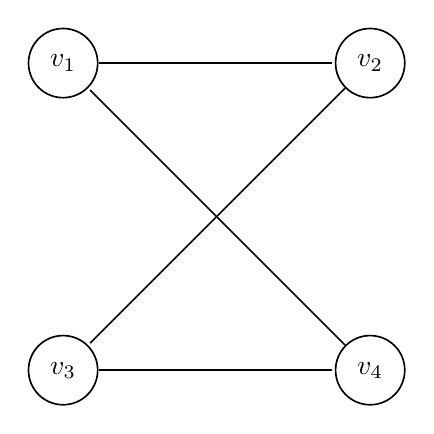
\begin{tikzpicture}[
    > = , % arrow head style
    shorten > = 1pt, % don't touch arrow head to node
    auto,
    node distance = 3cm, % distance between nodes
    semithick % line style
    ]

    \tikzset{every state}=[
    draw = black,
    thick,
    fill = black,
    minimum size = 1mm
    ]

    \node[state] (v1) {$v_1$};
    \node[state] (v2) [right=of v1] {$v_2$};
    \node[state] (v3) [below =of v1] {$v_3$};
    \node[state] (v4) [below =of v2] {$v_4$};
  
    \path[->] (v1) edge  node[]{}(v2);
    \path[->] (v2) edge  node[]{} (v3);
    \path[->] (v3) edge  node[]{}(v4);
    \path[->] (v4) edge  node[]{}(v1);
\end{tikzpicture}
\end{example}
There are many other examples of graphs, one of them being the complete graph on $\mathit{n}$ vertices.
\begin{definition}[Complete Graph]
\label{Complete Graph}
A graph G(V,E) is said to be complete if $\forall$ v,w $\in$ V v $\neq$ w, v is adjacent to w. The complete graph on n vertices is denoted by $K_n$. \normalfont{\cite{complete_graphs}}
\end{definition}
Given any graph $\mathit{G(V,E)}$, one can also define concepts that lie within G, one of them being a path.
\begin{definition}[Path]
\label{Path}
Given a graph G(V,E), a path in G joining any 2 vertices u,v $\in$ V, is a sequence of vertices u = $u_1$, $u_2$, ...,$u_n$ = v in which no vertex is repeated and, $\forall$ $u_i$,$u_{i+1}$ i $\in$ [n-1], \{$u_i,u_{i+1}\}$ $\in$ E {\normalfont{\cite{thompson}}}. A path on n vertices is denoted by $P_n$.
\end{definition}
Definition \ref{Path} can now be used to define cycles and connectivity in a graph.
\begin{definition}[Connected Graph]
\label{connectedgraph}
A graph G(V,E) is said to be connected if $\forall$ u,v $\in$ V u $\neq$ v, u and v are joined by a path. \normalfont{\cite{connected}}
\end{definition}
\begin{definition}[Cycle]
\label{cycle}
Given a graph G(V,E), a cycle in G is a path $P_n$ n $\geq$ 4, such that, the starting vertex and the end vertex are equal. \normalfont{\cite{cycle}} 
\end{definition}
By definitions \ref{Path}, \ref{cycle} above, it is clear that a cycle is a special instance of a path, with the only difference being that in a cycle, the first vertex and the last vertex are equal. Another thing worth mentioning is that according to definitions \ref{Path} and \ref{cycle}, cycles and paths are sequences of vertices and not actual graphs. However, this is not the case because they can be represented easily as graphs. For example, given the path/cycle $\mathit{u_1, u_2, ...,u_n}$ a new graph $\mathit{G(V,E)}$ can be created such that, $\mathit{V(G)= \{ u_1, u_2, ..., u_n\}}$ and $\mathit{E(G) = \{ \{u_i, u_{i+1}\} : i \in [n-1]\}}$. For example, consider the cycle v1 v2 v3 v4 v1, then the graph $\mathit{G(V,E)}$ $\mathit{V(G)= \{ v_1, v_2, v_3, v_4\}}$ \\$\mathit{E(G) = \{ \{v_1, v_2\}, \{v_2, v_3\}, \{v_3, v_4\}, \{v_4, v_1\} \}}$ depicted in example \ref{Example 1}, is the graph representing this cycle. Since this construction can be done, cycles/paths will be treated as both graphs and sequences in this thesis. This will later be useful when defining Hamiltonian cycles. For better understanding of definitions \ref{Complete Graph}, \ref{Path}, \ref{connectedgraph}, \ref{cycle} example \ref{example3} is constructed.
\begin{example}
\label{example3}
{\normalfont{Consider the graph}} G(V,E) {\normalfont{below:}}\\
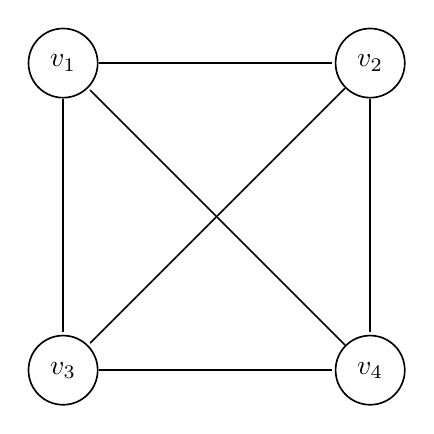
\begin{tikzpicture}[
    > = , % arrow head style
    shorten > = 1pt, % don't touch arrow head to node
    auto,
    node distance = 3cm, % distance between nodes
    semithick % line style
    ]

    \tikzset{every state}=[
    draw = black,
    thick,
    fill = black,
    minimum size = 1mm
    ]

    \node[state] (v1) {$v_1$};
    \node[state] (v2) [right=of v1] {$v_2$};
    \node[state] (v3) [below =of v1] {$v_3$};
    \node[state] (v4) [below =of v2] {$v_4$};
  
    \path[->] (v1) edge  node[]{}(v2);
    \path[->] (v1) edge  node[]{}(v3);
    \path[->] (v2) edge  node[]{} (v3);
    \path[->] (v3) edge  node[]{}(v4);
    \path[->] (v2) edge  node[]{}(v4);
    \path[->] (v4) edge  node[]{}(v1);
\end{tikzpicture}
\\
{\normalfont{Since every vertex in}} G {\normalfont{is adjacent to every other vertex, }}G {\normalfont{must be complete. Therefore, it must also be connected because, there is a path}} $P_2$ {\normalfont{between any 2 distinct vertices of}} G{\normalfont{. This graph is denoted by}} $K_4$ {\normalfont{since it is the complete graph on 4 vertices.}}\\
{\normalfont{Some examples of paths in}} G {\normalfont{are:}}\\
1. $v_1$ $v_2$ $v_3$ $v_4$\\
2. $v_1$ $v_4$\\
3. $v_4$ $v_3$ $v_1$\\
{\normalfont{Some examples of cycles in}} G {\normalfont{are:}}\\
1. $v_1$ $v_2$ $v_3$ $v_4$ $v_1$\\
2. $v_1$ $v_4$ $v_2$ $v_3$ $v_1$\\
3. $v_4$ $v_3$ $v_1$ $v_4$\\
\end{example}
Another important terminology is that of subgraphs. 
\begin{definition}[Subgraph]
\label{subgraph}
Given a graph G(V,E) and a graph H($V^\prime$,$E^\prime$), H is a subgraph of G if $V^\prime$ $\subseteq$ V and $E^\prime$ $\subseteq$ E.  \normalfont{\cite{harris_hirst_mossinghoff_2008}}
\end{definition}
After defining some important concepts, the next step is to extend definition \ref{Graph} to define another class of graphs called weighted graphs. It must be noted that all definitions presented so far apply also to weighted graphs.
\begin{definition}[Weight Function]
\label{Weighted Function}
Given a graph G(V,E) a weight function is a function f : E $\mapsto$ $\real$ {\normalfont{\cite{harris_hirst_mossinghoff_2008}}}. The real numbers assigned to each edge are called weights.
\end{definition}
\begin{definition}
\label{Weighted Graph}
A weighted graph is a graph G(V,E) with a weight function f {\normalfont{\cite{harris_hirst_mossinghoff_2008}}}. This is denoted by the triple G(V,E,f). 
\end{definition}
According to Bondy and Murty \cite{bondy_murty_1982}, weighted graphs occur regularly in applied graph theory. For example, a railway network can be represented by a weighted graph were, the vertices are the set of towns in the railway network, and there are edges between 2 vertices in the graph if there is a direct route from one town to another, without visiting other towns in the process. In addition to that, the shortest path between 2 towns in the network may be required. It is clear that in order to try and solve such problems, the total weight of a subgraph must first be defined.
\begin{definition}[Weight of a Subgraph]
\label{weightofasubgraph}
Given a weighted graph G(V,E,f), the total weight of any subgraph  H($V^\prime$,$E^\prime$,f) of G is: $$\sum_{e \in E^\prime}^{} f(e) $$. \normalfont{\cite{bondy_murty_1982}}
\end{definition}
It is important to note that by definition \ref{subgraph}, any weighted graph G is a subgraph of itself, therefore, it's weight can be calculated. This is highlighted in Example \ref{example4} below.
\begin{example}
\label{example4}
{\normalfont{Consider the weighted graph}} G(V,E,f) {\normalfont{such that,}} G(V,E) {\normalfont{ is the graph in example \ref{example3} with weight function}} f {\normalfont{such that}},\\
f(\{$v_1, v_2\}$) = 4\\
f(\{$v_1, v_3\}$) = 5\\
f(\{$v_2, v_3\}$) = 2\\
f(\{$v_3, v_4\}$) = 10\\
f(\{$v_2, v_4\}$) = 4\\
f(\{$v_4, v_1\}$) = 7\\
{\normalfont{Then according to definition \ref{weightofasubgraph}, the weight of}} G {\normalfont{is 32.}}\\
\end{example}
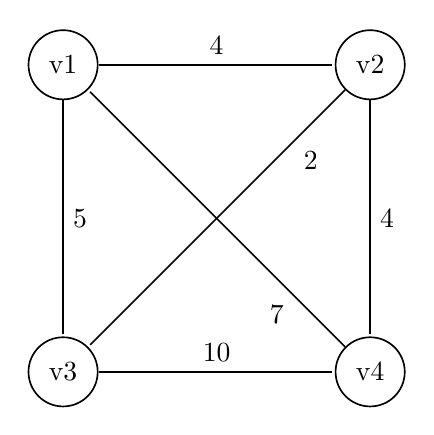
\begin{tikzpicture}[
    > = , % arrow head style
    shorten > = 1pt, % don't touch arrow head to node
    auto,
    node distance = 3cm, % distance between nodes
    semithick % line style
    ]

    \tikzset{every state}=[
    draw = black,
    thick,
    fill = white,
    minimum size = 1mm
    ]
    \node[state] (v1) {v1};
    \node[state] (v2) [right=of v1] {v2};
    \node[state] (v3) [below =of v1] {v3};
    \node[state] (v4) [below =of v2] {v4};
  
    \path[->] (v1) edge  node[]{4}(v2);
    \path[->] (v1) edge  node[]{5}(v3);
    \path[->] (v2) edge  node[pos=0.2,below right]{2} (v3);
    \path[->] (v3) edge  node[]{10}(v4);
    \path[->] (v2) edge  node[]{4}(v4);
    \path[->] (v4) edge  node[pos=0.2,below left]{7}(v1);
\end{tikzpicture}\\
\\
According to Guichard \cite{guichard_2018}, trees are another useful class of graphs.
\begin{definition}[Tree]
\label{tree}
A tree is a connected graph with no cycles. \normalfont{\cite{guichard_2018}}
\end{definition}
Having defined much of the basic graph theoretic concepts, it is now time to define harder concepts that use previous definitions. It is important to note that these concepts can be applied to both weighted and unweighted graphs.
\begin{definition}[Spanning Subgraph]
\label{spanning subgraph}
H($V^\prime$,$E^\prime$) is a spanning subgraph of G(V,E) if H is a subgraph of G and $V^\prime$ = V. \normalfont{\cite{ray_2013}}
\end{definition}
There are many spanning subgraphs, however the ones that are relevant to this thesis are spanning trees and spanning cycles, the latter mostly known as Hamiltonian cycles.
\begin{definition}[Spanning Tree]
A graph H is a spanning tree of G if H is a tree and H is a spanning subgraph of G. \normalfont{\cite{ray_2013}}
\label{spanning tree}
\end{definition}
\begin{definition}[Hamiltonian Cycle]
\label{hamiltonian cycle}
Given a graph G, c is a Hamiltonian cycle in G if c is a cycle and c is a spanning subgraph of G. Also, a graph that contains a Hamiltonian cycle is called a Hamiltonian graph. \normalfont{\cite{weisstein_2018}}
\end{definition}
It is worth mentioning that definition \ref{hamiltonian cycle} holds because, cycles can be represented as graphs by the construction discussed earlier. What follows now is an example that illustrates better definitions \ref{spanning subgraph}, \ref{spanning tree} and \ref{hamiltonian cycle}. 
\begin{example}
\label{example5}
{\normalfont{Let}} G {\normalfont{be the graph in example \ref{example4}. Then, according to definition \ref{spanning subgraph}, the 2 graphs below are 2 spanning subgraphs of}} G {\normalfont{because, they contain all the vertices of}} G {\normalfont{and are subgraphs of }}G .\\
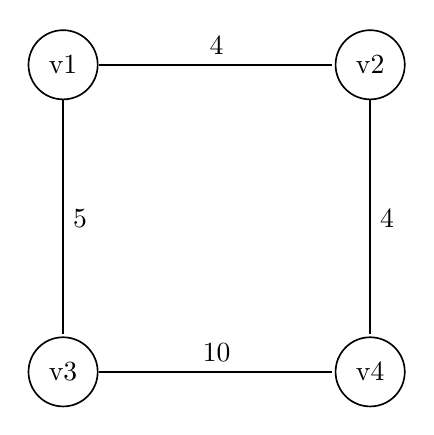
\begin{tikzpicture}[
    > = , % arrow head style
    shorten > = 1pt, % don't touch arrow head to node
    auto,
    node distance = 3cm, % distance between nodes
    semithick % line style
    ]

    \tikzset{every state}=[
    draw = black,
    thick,
    fill = white,
    minimum size = 1mm
    ]
    \node[state] (v1) {v1};
    \node[state] (v2) [right=of v1] {v2};
    \node[state] (v3) [below =of v1] {v3};
    \node[state] (v4) [below =of v2] {v4};
  
    \path[->] (v1) edge  node[]{4}(v2);
    \path[->] (v1) edge  node[]{5}(v3);
    \path[->] (v3) edge  node[]{10}(v4);
    \path[->] (v2) edge  node[]{4}(v4);
\end{tikzpicture}\\
\\
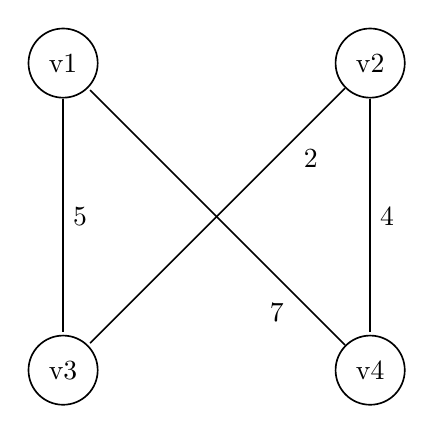
\begin{tikzpicture}[
    > = , % arrow head style
    shorten > = 1pt, % don't touch arrow head to node
    auto,
    node distance = 3cm, % distance between nodes
    semithick % line style
    ]

    \tikzset{every state}=[
    draw = black,
    thick,
    fill = white,
    minimum size = 1mm
    ]
    \node[state] (v1) {v1};
    \node[state] (v2) [right=of v1] {v2};
    \node[state] (v3) [below =of v1] {v3};
    \node[state] (v4) [below =of v2] {v4};
  
    \path[->] (v1) edge  node[]{5}(v3);
    \path[->] (v2) edge  node[pos=0.2,below right]{2} (v3);
    \path[->] (v2) edge  node[]{4}(v4);
    \path[->] (v4) edge  node[pos=0.2,below left]{7}(v1);
\end{tikzpicture}\\
{\normalfont{It must also be said that by definition \ref{hamiltonian cycle}, the above 2 graphs are Hamiltonian cycles because, they are spanning subgraphs of}} G {\normalfont{and are graphs that represent cycles in G. Since the above graphs are subgraphs of }}G{\normalfont{, by definition \ref{weightofasubgraph}, their weight can be calculated by summing up the weights of the edges. Thus, the Hamiltonian cycles above have weight 23 and 18 respectively.}}\\
{\normalfont{Given the same graph }}G{\normalfont{ in example \ref{example4}, the 2 graphs below are spanning trees of }}G{\normalfont{ of weight 18 and 19 respectively.}}\\
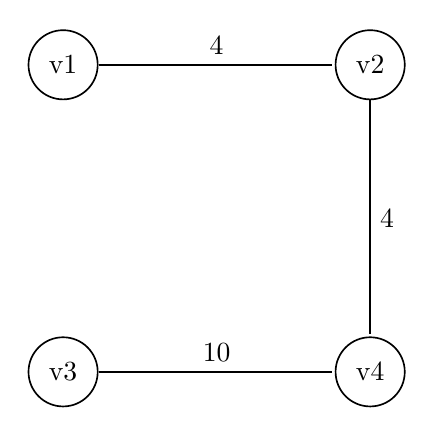
\begin{tikzpicture}[
    > = , % arrow head style
    shorten > = 1pt, % don't touch arrow head to node
    auto,
    node distance = 3cm, % distance between nodes
    semithick % line style
    ]

    \tikzset{every state}=[
    draw = black,
    thick,
    fill = white,
    minimum size = 1mm
    ]
    \node[state] (v1) {v1};
    \node[state] (v2) [right=of v1] {v2};
    \node[state] (v3) [below =of v1] {v3};
    \node[state] (v4) [below =of v2] {v4};
  
    \path[->] (v1) edge  node[]{4}(v2);
    \path[->] (v3) edge  node[]{10}(v4);
    \path[->] (v2) edge  node[]{4}(v4);
\end{tikzpicture}\\
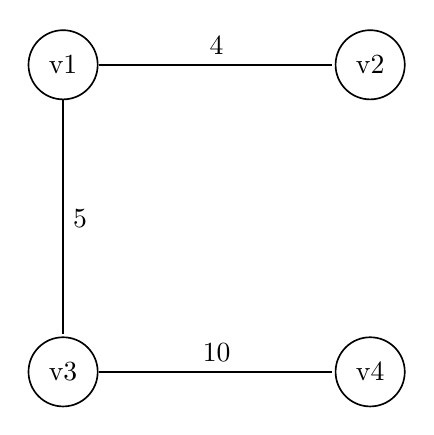
\begin{tikzpicture}[
    > = , % arrow head style
    shorten > = 1pt, % don't touch arrow head to node
    auto,
    node distance = 3cm, % distance between nodes
    semithick % line style
    ]

    \tikzset{every state}=[
    draw = black,
    thick,
    fill = white,
    minimum size = 1mm
    ]
    \node[state] (v1) {v1};
    \node[state] (v2) [right=of v1] {v2};
    \node[state] (v3) [below =of v1] {v3};
    \node[state] (v4) [below =of v2] {v4};
  
    \path[->] (v1) edge  node[]{4}(v2);
    \path[->] (v1) edge  node[]{5}(v3);
    \path[->] (v3) edge  node[]{10}(v4);
\end{tikzpicture}\\
{\normalfont{This example also shows that within the same weighted graph, there could be multiple Hamiltonian cycles and spanning trees of different weight.}}
\end{example}
Having defined Hamiltonian cycles and spanning trees, it is natural to ask whether there are necessary and sufficient conditions in a graph that guarantee that the graph is Hamiltonian or that it contains a spanning tree as subgraph. In fact, these necessary and sufficient conditions are known for a graph to have a spanning tree.
\begin{theorem}
A graph G has a spanning tree $\iff$ it is connected.
\label{spanningtreetheorem}
\end{theorem} 
\begin{proof}
($\implies$) Let $\mathit{G(V,E)}$ be a graph having a spanning tree $\mathit{T(V^\prime,E^\prime)}$ as one of it's subgraphs. Let $\mathit{v1, v2}$ $\in$ $\mathit{V}$. Since, $\mathit{T}$ is a spanning tree of $\mathit{G}$, then, $\mathit{T}$ is a spanning subgraph of $\mathit{G}$. Thus, $\mathit{v1, v2}$ $\in$ $V^\prime$. Also, since $\mathit{T}$ is a tree, $\mathit{T}$ must be connected. Therefore, $\exists$ a path $\mathit{P}$ joining vertices $\mathit{v1}$ and $\mathit{v2}$ in $\mathit{T}$. But since $\mathit{T}$ is a subgraph of G, then $\mathit{P}$ is also a path in $\mathit{G}$. Therefore $\mathit{G}$ must be connected.\\
($\Leftarrow$) Conversely, let $\mathit{G(V,E)}$ be a connected graph. Then, if $\mathit{G}$ has no cycles, $\mathit{G}$ itself must be a spanning tree. If $\mathit{G}$ has cycles, delete an edge from a cycle in $\mathit{G}$. Clearly, the resultant graph is still connected and contains one less cycle. Repeat this procedure untill no more cycles are left in the graph. Then, the resultant graph $\mathit{G^\prime}$ would be a connected subgraph of $\mathit{G}$ having no cycles(i.e a tree). Also, since no vertex was deleted from $\mathit{G}$, $\mathit{G^\prime}$ is a spanning subgraph of $\mathit{G}$. Therefore $\mathit{G^\prime}$ is a spanning tree of $\mathit{G}$.
\end{proof}
Theorem \ref{spanningtreetheorem} confirms that for a graph to have a spanning tree, the graph must be connected and vice-versa. Thus, for spanning trees, the necessary and sufficient condition is connectivity. 
\newpage
\section{The Travelling Salesman Problem}
\subsection{Heuristics}
\subsection{The Ant Colony Algorithm}
\newpage
\section{Experimental Data}
\newpage
\section{Conclusion}
\newpage
\bibliography{bibliography}
\bibliographystyle{IEEEtran}
\end{document}